\section{Introduction}
\emph{Convex optimization} is a subfield of optimization in which we are interested in minimizing a convex function over a convex set. Compared to the general optimization problem, convex optimization solves a simpler problem, allowing to develop efficient algorithms.

\subsection{Why Convex Optimization?}
Convex optimization is a very mature field, with a lot of theory and algorithms developed over the years. \say{Generic} working recipes are available for a wide range of problems, and the algorithms are often very efficient. Moreover, the theory of convex optimization is very well understood, and we can often prove that the algorithms converge to the optimal solution.

\subsection{Historical perspective}
There is a general belief that convex optimization problems are simple. While this is often true, this is not correct in general. Historically, non-linear problems were seen as hard, compared to the easier linear ones. The modern perspective differs:
\begin{center}
    \say{In fact the great watershed in optimization isn't between linearity and nonlinearity,\\ but convexity and nonconvexity.}\footnote{R. T. Rockafellar. “Lagrange multipliers and optimality.” SIAM Review, 1993.}
\end{center}
Papers such as \say{¨roblem Complexity and Method Efficiency in Optimization.} by Nemirovskii and Yudin in 1979, or \say{Interior-Point Polynomial Methods in Convex Programming.} by Nesterov and Nemirovskii in 1994, progressively developed a robust theory and efficient algorithms for convex optimization.

The simplex algorithm, developed by Dantzig in 1949, solves linear programmin problems in exponential time for the worst case. However, it is very efficient in most cases. The ellipsoid method is used since Khachiyan in 1979 to show the polynomial complexity of LP. It is only since Karmakar in 1984 that an efficient polynomial time algorithm for LP was developed, using interior point methods.

The same interior point methods (IPM) were used by Nesterov and Nemirovskii to develop efficient algorithms for a larger class of structure convex problems. The self-concordance analysis that they introduce extends the polynomial time complexity proof for LPs; most operations that preserve convexity also preserve self-concordance.

\subsection{Algorithmic persepective}
\subsubsection{Interior Point Methods}
Interior point methods (IPM) essentially solved once and for all a broad range of medium-scale convex programs. For large-scale problems, computing a single Newton step is often too expensive.

\subsubsection{First-order methods}
First-order methods are often used for large-scale problems. They are based on the gradient of the function, and are often very efficient. The dependence on precision becomes polynomial $O(1/\varepsilon^\alpha)$, and not logarithmic $O(\log(1/\epsilon))$ as in IPM. This is acceptable in many applications (statistics, machine learning, etc.). It runs a much larger number of iterations, but each iteration is much cheaper. The lack of Hessian requires significantly less memory and CPU costs per iteration.

On the other hand, there is no unified analysis (as self-concordance for IPM) for first-order methods: there is therefore a huge jungle of disparate methods; the algorithmic choices are stricly constrained by the problem structure.

\subsubsection{Time and error}
In many optimization schemes, the usages depend on the application requirements (such as the target precision, the time budget, memory budget, etc.).
\begin{figure}[H]
    \centering
    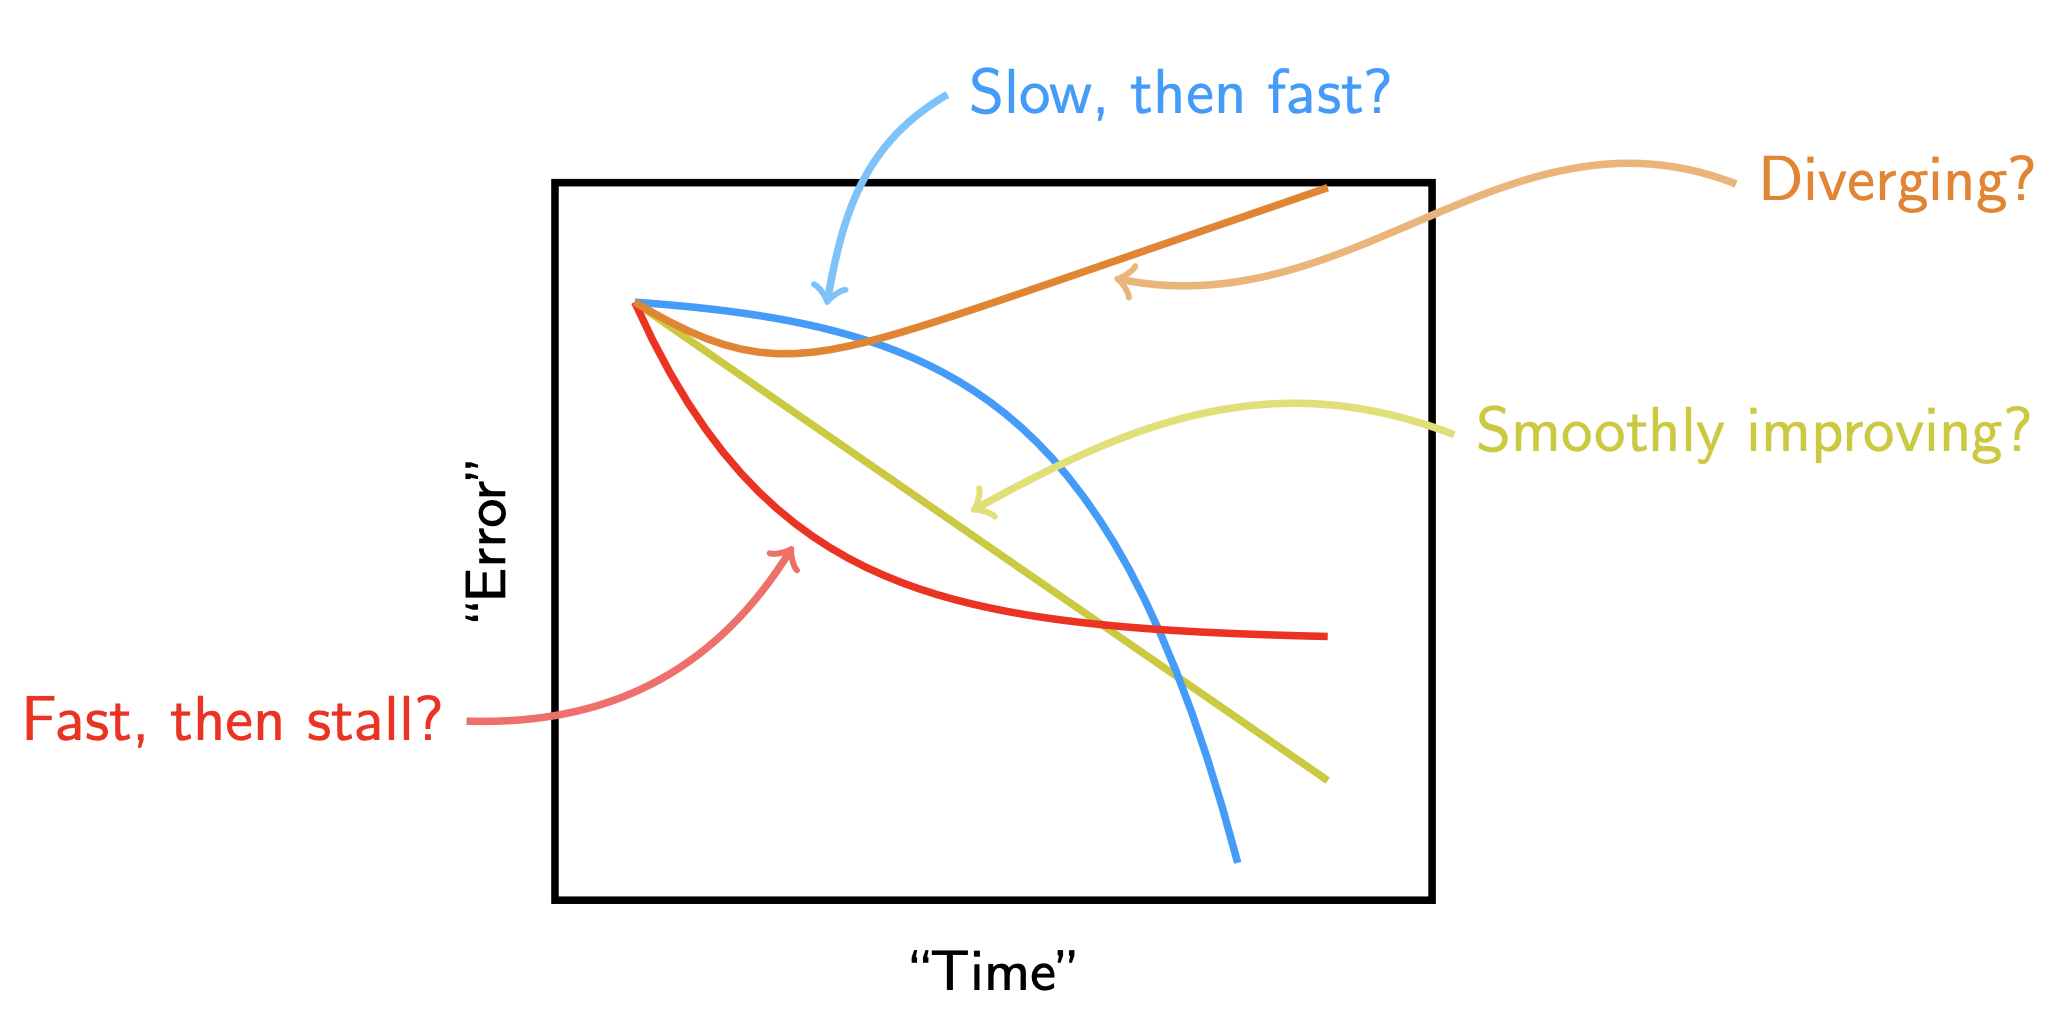
\includegraphics[width=0.7\textwidth]{introduction/graph.png}
\end{figure}
Diverse algorithms have different trade-offs between time and error.

\subsection{Exploiting the problem structure}
Formally, our target is to solve a problem of the form:
\begin{equation*}
    \minimize_{x\in C} f(x)
\end{equation*}
To solve it efficiently, we must exploit the knowledge about the problem properties. What is known about $f$ and $C$? What can I efficiently compute and use to minimize $f$ over $C$? What am I aiming for?

For instance, the ability to compute gradients of $f$, the Hessian, or to solve Newton systems can be crucial. The structure of $C$ can also be very important: can I project onto $C$? What is the target accuracy. This kind of questions drives the choice for optimization schemes.